\subsection{Autopilot}
	\begin{figure}[H]
		\centering
		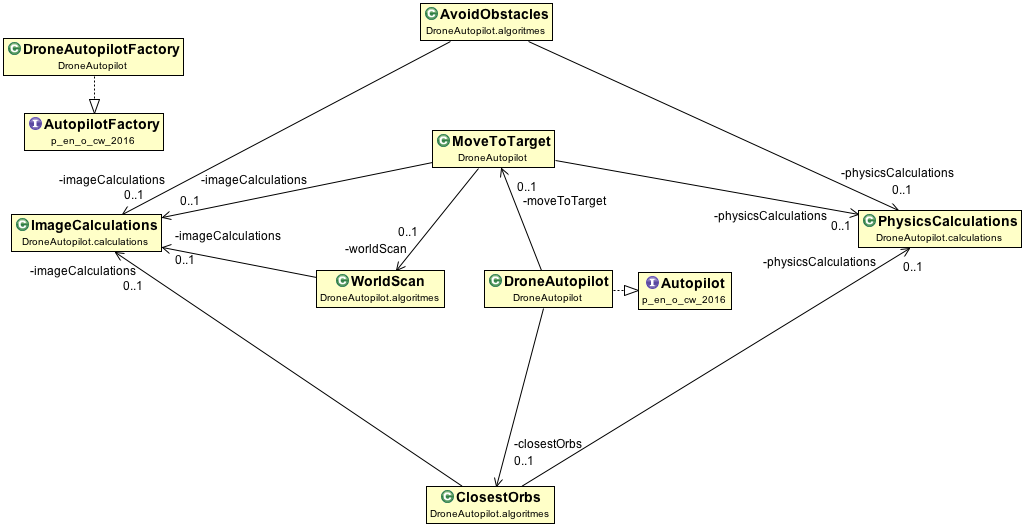
\includegraphics[width=1\textwidth]{AutopilotDiagram.png}
		\caption{Dit klassendiagram geeft de basisstructuur weer van de Autopilot. \textit{MoveToTarget} is het vitale gedeelte van de Autopilot. Deze klasse baseert zich op de berekeningen in \textit{ImageCalculations} en \textit{PhysicsCalculations}. Ook Figuren \ref{fig: mission} en \ref{fig: control} horen hierin verwerkt te zijn. Echter voor een overzichtelijk beeld van het geheel wordt dit niet gedaan. }
	\end{figure}
	\begin{figure}[H]
		\centering
		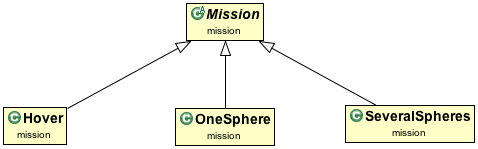
\includegraphics[width=0.6\textwidth]{MissionDiagram.png}
		\caption{De \textit{Mission}-structuur kan gemakkelijk worden uitgebreid voor extra mijlpalen. In \textit{Mission} wordt de \texttt{execute()} steeds ingevuld met \textit{MoveToTarget} in combinatie met de gewenste strategie.}
		\label{fig: mission}
	\end{figure}
	\begin{figure}[H]
		\centering
		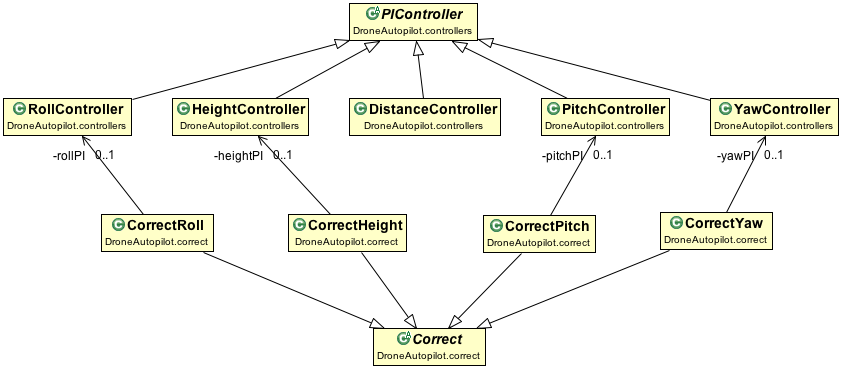
\includegraphics[width=1\textwidth]{ControlDiagram.png}
		\caption{De \textit{Controllers} geven de wiskundige implementatie weer, terwijl de \textit{Correctors} zorgen voor de correcte implementatie binnen het systeem. De \textit{Correctors} worden in combinatie met \textit{MoveToTarget} gebruikt om het gewenste doel (één bol of verschillende bollen) te bereiken.}
		\label{fig: control}
	\end{figure}
\subsection{Virtual Testbed}
	\begin{figure}[H]
		\centering
		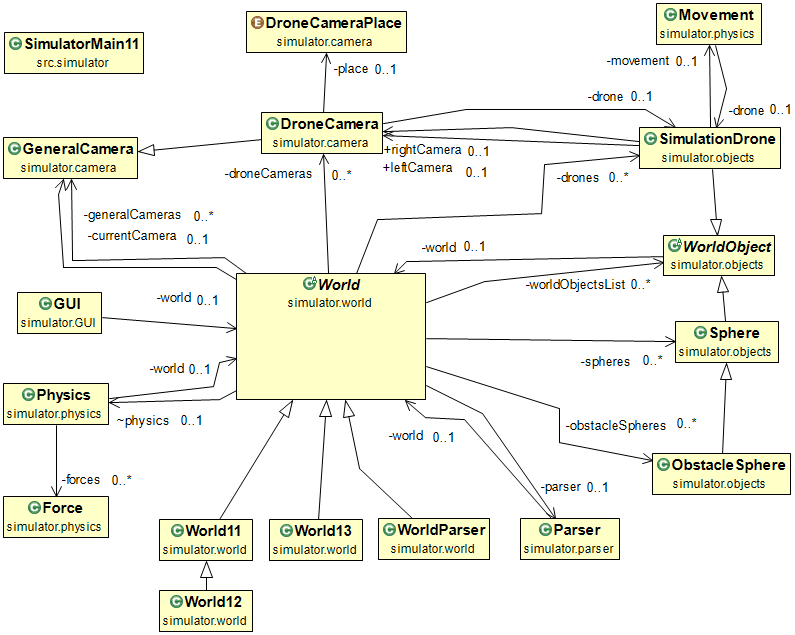
\includegraphics[width=1\textwidth]{Simulator.png}
		\caption{Dit klassendiagram geeft de basisstructuur weer van het Virtual Testbed. Centrale klassen  zijn \textit{World}, \textit{WorldObject} en \textit{GeneralCamera}. Voor uitgebreide uitleg wordt verwezen naar sectie \ref{sec:SoftwareVirtualTestbed}.}
	\end{figure}